\chapter{Lecture 22 - Classical PDEs and BVPs}
\label{ch:lec22}
\section{Objectives}
\begin{itemize}
\item Describe three important PDEs: heat equation, wave equation, and Laplace equation.
\item Describe the physical meaning of common boundary conditions.
\item Discuss important modifications to the three equations to incorporate additional physical phenomena.
\end{itemize}

\section{The Heat Equation}
The time-dependent heat equation in one spatial dimension is given in Equation \ref{eq:heat-eq}:
\begin{equation}
\frac{\partial u}{\partial t} = \alpha^2\frac{\partial^2 u}{\partial x^2}, \ \ \alpha > 0, \ \ a<x<b
\label{eq:heat-eq}
\end{equation}
where $\alpha^2$ corresponds to thermal diffusivity which, in turn is given in Equation \ref{eq:thermal-diffusivity}:
\begin{equation}
\alpha^2 = \frac{k}{\rho c_p}
\label{eq:thermal-diffusivity}
\end{equation}
where $k$ is thermal conductivity, $\rho$ is the density, and $c_p$ is the specific heat at constant pressure and the dependent variable $u$ is the temperature.  All of these material properties must be positive for physically meaningful materials and, for the time being at least, we will consider all of these properties to be constant.\sidenote{This is a very important assumption mathematically and it is also untrue for relevant materials.  The thermal conductivity of most materials is temperature dependent as is the density and specific heat.  If we allowed for this bit of realism to slip into our mathematical analysis, however, the differential equation would become nonlinear---$\alpha$ would become a function of the dependent variable $u$---and we would not be able to solve it with methods taught in this class. Tools based on the finite element method such as MOOSE and COMSOL are specifically designed to deal with this sort of nonlinearity.}

\newthought{We will not} delve into the derivation of Equation \ref{eq:heat-eq}; this is left for your class in heat transfer.  Suffice it to say here that the equation is a mathematical expression of conservation of energy.  The following assumptions are incorporated into this expression:
\begin{enumerate}
\item Heat is flowing in one spatial direction only.  This is the reason why the equation is only a function of $x$.  Think of this as heat flowing in a wire.
\item Since heat is assumed to only flow in the $x$-direction, you should assume that the lateral surfaces of this wire are insulated.  
\item We assume that no heat is generated in the domain.
\item We assume that the material is homogeneous.
\item We also assumed a particular relationship between heat flow and the temperature gradient:\marginnote[-2.0cm]{Strictly speaking, Equation \ref{eq:heat-eq-constituitive} should reference an outward-pointing unit-normal vector.  In a more generic case we would express the relationship as:
\begin{equation*}
q = -k \nabla u \cdot \hat{n}
\end{equation*}
where $\hat{n}$ is the outward-pointing unit normal on the surface through which the heat flux flows and, of course, $\nabla u$, is the temperature gradient.  In a one-dimensional problem like this, $\nabla u$ reduces to $\sfrac{\partial u}{\partial x}$.  To get the physics right (or, more specifically, to get the sign of the heat flux correct) for a particular problem, however, one will need to remember the dot-product with the outward-pointing unit normal.
}
\begin{equation}
q = -k\frac{\partial u}{\partial x}
\label{eq:heat-eq-constituitive}
\end{equation}
where $q$ is the \emph{heat flux}.  Relationships such as given in Equation \ref{eq:heat-eq-constituitive} are referred to as \emph{constitutive} relationships.
\end{enumerate}  

\newthought{To be fully} meaningful as an initial boundary value problem (IBVP), Equation \ref{eq:heat-eq} must be accompanied by an initial condition---say an initial temperature profile, $u(x,0) = f(x)$---and two boundary conditions.  We categorize the boundary conditions into three types:

\vspace{0.5cm}

\noindent\textbf{Type 1:} These are also called \emph{Dirichlet boundary conditions}.\sidenote{Named after the German mathematician Peter Gustav Lejeune Dirichlet who was known as a popular instructor at the Prussian Military Academy in the mid 19\textsuperscript{th} century. He is also famous for having first established the convergence proofs that we have cited for Fourier series and he also studied and proved a unique solution for the first boundary value problem.  That, to the best of my knowledge, is why this boundary condition type is named for him.} These conditions apply to the dependent variable itself.  For example:
\begin{equation*}
u(a) = T_a, \ \ u(b) = f(t)
\end{equation*}

\vspace{0.5cm}

\noindent\textbf{Type 2:} These are also called \emph{Neumann} boundary conditions and they apply to the \emph{derivative} of the dependent variable.  For example:
\begin{equation*}
\frac{\partial u}{\partial x}\Bigl|_{x=a} = 0
\end{equation*}
For the heat equation a homogeneous boundary condition of this type would indicate insulation at a boundary.\sidenote{Insulation implies no heat transfer through a surface---i.e. no heat flux.  Since heat flux is proportional to $\nabla u \cdot \hat{n}$ this implies, for one-dimensional problems, that $\sfrac{\partial u}{\partial x} = 0$.}

\vspace{0.5cm}

\noindent\textbf{Type 3:} These are called \emph{mixed} or \emph{Robin} boundary conditions and they apply to \emph{both} the dependent variable and its derivative.  For example:
\begin{equation*}
\frac{\partial u}{\partial x}\Bigl|_{x=b} = -h\left(u(b,t)-u_m\right), \ \ h>0
\end{equation*}
where, in this case, $u_m$ is a constant reference temperature of the surrounding medium and $h$ is a convective heat transfer coefficient.  This boundary condition would correspond to convective heat transfer at the boundary in which the heat flux is proportional ($h$ being the proportionality constant) to the difference in temperature between the boundary surface and the surrounding medium.

\section{Wave Equation}

The wave equation is given by Equation \ref{eq:wave}:
\begin{equation}
\frac{\partial^2 u}{\partial t^2} = \alpha^2 \frac{\partial^2 u}{\partial x^2}, \ \ \alpha>0, \ \ a<x<b
\label{eq:wave}
\end{equation}
where $\alpha^2 = \frac{T}{\rho}$ and $T$ is tension and $\rho$ is density.\sidenote{The variable $\alpha$ is also often referred to as the \emph{wave speed}.}  The dependent variable $u$ refers to lateral displacement of the string and $t$ is time.
\begin{marginfigure}
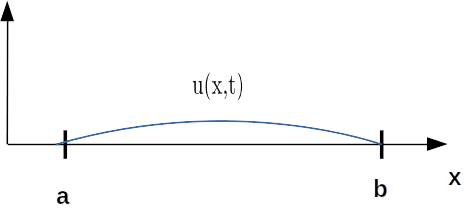
\includegraphics{wave_eq_disp.png}
\end{marginfigure}

This equation is derived as a mathematical expression of mechanical equilibrium of an elastic string held under tension.  The assumptions built-in to this derivation include:
\begin{enumerate}
\item The string is ``perfectly flexible.'' 
\item The string is homogeneous.
\item Displacements in the string are small relative to the string length.
\item Tension is constant; and
\item there are no other forces acting on the string.
\end{enumerate}
A properly stated boundary value problem based on the wave equation will have two boundary conditions.  For this course we will usually apply Dirichlet boundary conditions but others are possible.  Since the equation is second-order in time we also need two temporal boundary conditions.  Typically these are given as the initial displacement, $u(x,0)=f(x)$, and initial velocity, $u_t(x,0)=g(x)$.

\section{Laplace Equation}
The Laplace equation in two dimensions in a Cartesian coordinate system is given by Equation \ref{eq:laplace-eq}:
\begin{equation}
\frac{\partial^2 u}{\partial x^2} + \frac{\partial^2 u}{\partial y^2} = 0
\label{eq:laplace-eq}
\end{equation}
The Laplace equation arises in studies of \emph{steady state} phenomena involving potentials such as: electrostatic potential, gravitational potential, velocity, and heat conduction.  The meaning of the dependent variable $u$, of course, depends upon what is being modeled.  

Equation \ref{eq:laplace-eq} can more concisely and generically be expressed using the Laplace operator $\nabla^2$.\marginnote[-2.0cm]{The Laplace operator $\nabla^2$ is short-hand for:

\begin{equation*}
\nabla^2 = \nabla \cdot \nabla 
\end{equation*}
where in Cartesian coordinates:
\begin{align*}
 \nabla &= \left\langle \frac{\partial}{\partial x}, \frac{\partial}{\partial y}, \frac{\partial}{\partial z} \right\rangle \\
 \nabla \cdot \nabla &= \left\langle \frac{\partial}{\partial x}, \frac{\partial}{\partial y}, \frac{\partial}{\partial z} \right\rangle \cdot \left\langle \frac{\partial}{\partial x}, \frac{\partial}{\partial y}, \frac{\partial}{\partial z} \right\rangle \\
 &= \frac{\partial^2}{\partial x^2} + \frac{\partial^2}{\partial y^2} + \frac{\partial^2}{\partial z^2} \\
&\text{also expressed as: } \\
\nabla^2 &= \bigtriangleup
\end{align*}

}
Using this notation, Equation \ref{eq:laplace-eq} could be written: $\nabla^2 u = 0$.  This same expression is valid for 1-, 2-, or 3-dimensional Cartesian coordinates but it is also valid for polar, cylindrical and spherical coordinates.  The specialization comes in the definition of $\nabla$.  We will address this further when we examine problems in those coordinate systems.

\section{Boundary Value Problems}
In all of the above cases, a full statement of the boundary value problem must include:
\begin{enumerate}
\item The partial differential equation,
\item all boundary conditions, and
\item initial conditions for time-dependent problems.
\end{enumerate}

\vspace{0.5cm}

\noindent\textbf{Example:} Wave Equation Boundary Value Problem.\marginnote{Note that, technically speaking, the PDE does not apply at the domain boundaries or at $t=0$.}
\begin{table}
\begin{tabular}{l l}
PDE & $ \frac{\partial^2 u}{\partial t^2} = \alpha^2 \frac{\partial^2 u}{\partial x^2}, \ \ 0<x<L, \ t>0$\\
 & \\
BCs: & $u(0,t) = 0, \ \ u(L,t) = 0, \ t>0$ \\
 & \\
ICs: & $u(x,0)=f(x), \ \ u_t(x,0)=g(x), \ \ 0<x<L$ \\
\end{tabular}
\end{table}

\subsection{Important Variations to Classic BVPs}
Both the heat equation and the wave equation incorporated several assumptions in the derivation.  If these assumptions are modified or eliminated we can still derive an equation but the form of the equation will change.  Some important variations are described here.

\newthought{In Equation \ref{eq:heat-eq-with-variations}} we show the heat equation in the case where there is an internal heat source and convection from lateral surfaces to a surrounding medium maintained at a constant temperature $u_m$:
\begin{equation}
\frac{\partial u}{\partial t} = \alpha^2 \frac{\partial^2 u}{\partial x^2} \underbrace{+ S(x,t)}_{\text{heat source}} \overbrace{- h(u-u_m)}^{\substack{\text{convection from} \\ \text{lateral surfaces}}}
\label{eq:heat-eq-with-variations}
\end{equation}
where $h$ is the convective heat transfer coefficient.

\newthought{In Equation \ref{eq:wave-eq-with-variations}} we show the wave equation in a case where we have an external force, damping and restoring forces.

\begin{equation}
\frac{\partial^2 u}{\partial t^2} = \alpha^2 \frac{\partial^2 u}{\partial x^2} \overbrace{+f(x,t)}^{\substack{\text{external}\\\text{force}}} \underbrace{-c\frac{\partial u}{\partial t}}_{\text{damping}}\overbrace{-ku}^{\substack{\text{restoring}\\ \text{force}}}
\label{eq:wave-eq-with-variations}
\end{equation}

\vspace{2.0cm}

\newthought{An important skill} that an engineer needs to develop is the ability to translate a description of a physical system into a properly formulated boundary value problem that you can solve.  The \emph{point} is be able to describe a system mathematically so that, by solving the math problem, you gain \emph{insight} into the behavior of the physical system.\marginnote{This is something that students in this class often struggle with.}  Here are a couple of examples to get started.

\vspace{0.15cm}

\noindent\textbf{Example: } Consider a rod of length $L$ that is insulated along its lateral surfaces.  There is heat transfer from the left end of the rod into a surrounding medium at temperature $20^{\circ}$ and the right end is insulated.  The initial temperature is $f(x)$ throughout.  We would like to know what the temperature distribution is as a function of time and space.  The corresponding BVP is:
\begin{table}
\begin{tabular}{l l}
PDE: & $\frac{\partial u}{\partial t}, \ \ 0<x<L, \ t>0 $ \\
& \\
BCs: & $\frac{\partial u}{\partial x}\Bigl|_{x=0} = -h(u(0,t)-20), \ \  \frac{\partial u}{\partial x}\Bigl|_{x=L} = 0, \ \ t>0$ \\
& \\
IC: & $u(x,0) = f(x), \ \ 0<x<L$ \\
\end{tabular}
\end{table}

\vspace{0.25cm}

\noindent\textbf{Example: } Consider a string of length $L$ held in tension.  The ends are secured to the $x-$axis, and the string is initially at rest on that axis.  An external vertical force proportional to the horizontal distance from the left end acts on the string for $t>0$.  The corresponding BVP is:
\begin{table}
\begin{tabular}{l l}
PDE: & $\frac{\partial^2 u}{\partial t^2} = \alpha^2 \frac{\partial^2 u}{\partial x^2} + hx, \ \ 0<x<L, \ t>0 $ \\
& \\
BCs: & $u(0,t)=0, \ \ u(L,t) = 0, \ t>0 $ \\
& \\
ICs: & $u(x,0) = 0, \ u_t(x,0) = 0, \ \ 0<x<L$ \\
\end{tabular}
\end{table}

\vspace{0.25cm}

\noindent\textbf{Example: } Consider a semi-infinite plate coinciding with the region $0 \le x \le \pi, \ \  y\ge 0.$  The left end is held at temperature $e^{-y}$, and the right end is held at temperature $100^{\circ}$C for $0 < y \le 1$ and $0^{\circ}$C for $y>1$.  The bottom of the plate, $y=0$, is held at temperature $f(x)$.  The corresponding BVP is:

\begin{table}
\begin{tabular}{l l}
PDE: & $\frac{\partial^2 u}{\partial x^2} + \frac{\partial^2 u}{\partial y^2} = 0, \ \ 0<x<\pi, \ y>0 $ \\
& \\
BCs: & $u(0,y) = e^{-y}, \ y>0, \ \ u(\pi,y) = \begin{cases} 100 & 0 < y \le 1 \\ 0 & y>1 \end{cases} $ \\
& $u(x,0) = f(x), \ \ 0<x<\pi $\\
\end{tabular}
\end{table}
One implicit constraint that may need to be applied in this cases is: $\lim_{y \to \infty} u(x,y) < \infty$. 
